\documentclass[
  onecolumn]{article}
\usepackage{amsmath,amssymb}
\usepackage{lmodern}


\usepackage{setspace}
\usepackage{iftex}
\ifPDFTeX
  \usepackage[T1]{fontenc}
  \usepackage[utf8]{inputenc}
  \usepackage{textcomp} % provide euro and other symbols
\else % if luatex or xetex
  \usepackage{unicode-math}
  \defaultfontfeatures{Scale=MatchLowercase}
  \defaultfontfeatures[\rmfamily]{Ligatures=TeX,Scale=1}
\fi
% Use upquote if available, for straight quotes in verbatim environments
\IfFileExists{upquote.sty}{\usepackage{upquote}}{}
\IfFileExists{microtype.sty}{% use microtype if available
  \usepackage[]{microtype}
  \UseMicrotypeSet[protrusion]{basicmath} % disable protrusion for tt fonts
}{}
\makeatletter
\@ifundefined{KOMAClassName}{% if non-KOMA class
  \IfFileExists{parskip.sty}{%
    \usepackage{parskip}
  }{% else
    \setlength{\parindent}{0pt}
    \setlength{\parskip}{6pt plus 2pt minus 1pt}}
}{% if KOMA class
  \KOMAoptions{parskip=half}}
\makeatother
\usepackage{xcolor}
\IfFileExists{xurl.sty}{\usepackage{xurl}}{} % add URL line breaks if available
\IfFileExists{bookmark.sty}{\usepackage{bookmark}}{\usepackage{hyperref}}
\hypersetup{
  pdftitle={Comparing Treatments for Amblyopia with a Synaptic Plasticity Model},
  pdfauthor={Brian S. Blais},
  colorlinks=true,
  linkcolor={blue},
  filecolor={blue},
  citecolor={blue},
  urlcolor={blue},
  pdfcreator={LaTeX via pandoc}}
\urlstyle{same} % disable monospaced font for URLs
\usepackage{graphicx}
\graphicspath{{resources/}}
\makeatletter
\def\maxwidth{\ifdim\Gin@nat@width>\linewidth\linewidth\else\Gin@nat@width\fi}
\def\maxheight{\ifdim\Gin@nat@height>\textheight\textheight\else\Gin@nat@height\fi}
\makeatother
% Scale images if necessary, so that they will not overflow the page
% margins by default, and it is still possible to overwrite the defaults
% using explicit options in \includegraphics[width, height, ...]{}
\setkeys{Gin}{width=\maxwidth,height=\maxheight,keepaspectratio}
% Set default figure placement to htbp
\makeatletter
\def\fps@figure{htbp}
\makeatother
\setlength{\emergencystretch}{3em} % prevent overfull lines
\providecommand{\tightlist}{%
  \setlength{\itemsep}{0pt}\setlength{\parskip}{0pt}}
\setcounter{secnumdepth}{2}
\ifLuaTeX
  \usepackage{selnolig}  % disable illegal ligatures
\fi
\newlength{\cslhangindent}
\setlength{\cslhangindent}{1.5em}
\newlength{\csllabelwidth}
\setlength{\csllabelwidth}{3em}
\newenvironment{CSLReferences}[2] % #1 hanging-ident, #2 entry spacing
 {% don't indent paragraphs
  \setlength{\parindent}{0pt}
  % turn on hanging indent if param 1 is 1
  \ifodd #1 \everypar{\setlength{\hangindent}{\cslhangindent}}\ignorespaces\fi
  % set entry spacing
  \ifnum #2 > 0
  \setlength{\parskip}{#2\baselineskip}
  \fi
 }%
 {}
\usepackage{calc}
\newcommand{\CSLBlock}[1]{#1\hfill\break}
\newcommand{\CSLLeftMargin}[1]{\parbox[t]{\csllabelwidth}{#1}}
\newcommand{\CSLRightInline}[1]{\parbox[t]{\linewidth - \csllabelwidth}{#1}\break}
\newcommand{\CSLIndent}[1]{\hspace{\cslhangindent}#1}

\title{Comparing Treatments for Amblyopia with a Synaptic Plasticity
Model}
\author{Brian S. Blais}
\date{}

\topmargin=-0.5in
\textheight=9.2in
\oddsidemargin=-0.2in
\evensidemargin=0.0in
\textwidth=6.90in
\parindent=30pt
\parskip=3pt
\headheight=15pt
\reversemarginpar
\marginparwidth=.75in
%
%
\renewcommand{\theequation}{\thesection.\arabic{equation}}
\newcommand{\doublesp}{\renewcommand{\baselinestretch}{2.0}}
\newcommand{\mediumsp}{\renewcommand{\baselinestretch}{1.6}}
\newcommand{\singlesp}{\renewcommand{\baselinestretch}{1.0}}
%
\pagestyle{myheadings}
\thispagestyle{empty}
\markright{\today}
\newlength{\figlen}
\setlength{\figlen}{3.7in}

\input stddefs.tex


\begin{document}
\maketitle

{
\hypersetup{linkcolor=}
\setcounter{tocdepth}{3}
\tableofcontents
}
\setstretch{1.5}
\hypertarget{preface}{%
\section*{Preface}\label{preface}}
\addcontentsline{toc}{section}{Preface}

These notes are produced with a combination of Obsidian
(\url{https://obsidian.md}), pandoc (\url{https://pandoc.org}), and some
self-styled python scripts
(\url{https://github.com/bblais/Amblyopia-Simulation/tree/main/Manuscript})

\hypertarget{software-installation}{%
\subsection*{Software Installation}\label{software-installation}}
\addcontentsline{toc}{subsection}{Software Installation}

The software is Python-based with parts written in Cython.

\begin{itemize}
\tightlist
\item
  Download the Anaconda Distribution of Python:
\end{itemize}

\url{https://www.anaconda.com/products/individual\#downloads}

\begin{itemize}
\tightlist
\item
  Download and extract the \emph{PlasticNet} package at:
\end{itemize}

\url{https://github.com/bblais/Plasticnet/archive/refs/heads/master.zip}

\begin{itemize}
\tightlist
\item
  Run the script \texttt{install.py}
\end{itemize}

\hypertarget{printable-versions}{%
\subsection*{Printable Versions}\label{printable-versions}}
\addcontentsline{toc}{subsection}{Printable Versions}

Printable versions of this report can be found on the GitHub site for
this project,

\begin{itemize}
\tightlist
\item
  \href{https://github.com/bblais/Amblyopia-Simulation/raw/main/Manuscript/docs/Comparing-Treatments-for-Amblyopia-with-a-Synaptic-Plasticity-Model.docx}{Microsoft
  Word version}
\item
  \href{https://github.com/bblais/Amblyopia-Simulation/raw/main/Manuscript/docs/Comparing-Treatments-for-Amblyopia-with-a-Synaptic-Plasticity-Model.pdf}{PDF
  version}
\end{itemize}

\hypertarget{introduction}{%
\section{Introduction}\label{introduction}}

These notes are an exploration of the problem of modeling Amblyopia and
its various treatments from an approach using synaptic plasticity
models. The process will involve constructing a simplified mechanism for
the development of amblyopic deficits and subsequently modeling both
monocular and binocular treatment protocols. The goal is to understand
the dynamics of the recovery from amblyopic deficits for the different
treatment protocols, to compare the effectiveness of each protocol, and
to explore their limitations. Ideally we would like to use these models
to inform future protocol parameters and perhaps suggest novel
treatments for amblyopia.

In this part we will explore the clinical basis for amblyopia and its
treatments. In the \ref{models-of-development-of-amblyopia} and
\ref{models-of-treatments-for-amblyopia} we will explore the models that
are used to describe the deficits from amblyopia and their treatment,
respectively.

\hypertarget{what-is-amblyopia}{%
\subsection{What is Amblyopia?}\label{what-is-amblyopia}}

Amblyopia is the most common cause of vision loss in children, caused by
refractive errors or misalignment of the eyes (Zárate and Tejedor,
2007).

\begin{itemize}
\tightlist
\item
  Visual acuity
\item
  Contrast sensitivity
\item
  Color
\item
  Depth (Stereopsis)
\item
  Motion
\item
  Visual fields
\end{itemize}

\hypertarget{how-is-it-treated}{%
\subsection{How is it Treated?}\label{how-is-it-treated}}

The current primary treatment is described in the \emph{Amblyopia
Preferred Practice Method} (Wallace et al., 2018). Treatments are
divided into two broad categories, monocular and binocular treatments.
Monocular treatments produce a competition between the two eyes by
treating only the fellow eye to that the amblyopic eye recovers.
Binocular treatments seek to stimulate both eyes in such a way that
binocular mechanisms can produce a recovery in the amblyopic eye.

\hypertarget{monocular-treatments}{%
\subsubsection{Monocular Treatments}\label{monocular-treatments}}

The most common treatment includes

\begin{enumerate}
\def\labelenumi{\arabic{enumi}.}
\tightlist
\item
  the optical correction of significant refractive errors
\item
  patching the dominant eye which forces the visual input to come from
  only the amblyopic eye.
\end{enumerate}

Although patching is the most common method of treatment, other methods
are described including pharmacology and technology (Gao et al., 2018;
Glaser et al., 2002; Jonathan M. Holmes et al., 2016b; Jonathan M.
Holmes et al., 2016a; Kelly et al., 2016; Li et al., 2015; Zárate and
Tejedor, 2007). These include,

\begin{enumerate}
\def\labelenumi{\arabic{enumi}.}
\setcounter{enumi}{2}
\tightlist
\item
  Pharmacological treatment with atropine drops in the fellow eye
\end{enumerate}

Each of these treatments only directly applies to the fellow eye and the
amblyopic eye is left untouched.

\hypertarget{binocular-treatments}{%
\subsubsection{Binocular Treatments}\label{binocular-treatments}}

There are some treatments which are administered to both eyes, making
them binocular treatments. The one that we will be addressing here use
virtual reality headsets(Xiao et al., 2020, 2022),

\begin{enumerate}
\def\labelenumi{\arabic{enumi}.}
\setcounter{enumi}{3}
\tightlist
\item
  Virtual reality input to both eyes, with contrast modification and/or
  dichoptic masks
\end{enumerate}

\hypertarget{mechanisms-for-amblyopia}{%
\subsection{Mechanisms for Amblyopia}\label{mechanisms-for-amblyopia}}

Since the unequal visual input to the brain can cause alterations in the
synaptic pathways leading to a disparity in ocular dominance (Birch,
2013), it is important to understand the possible synaptic effects
amblyopia can produce and how potential treatments will either help or
hinder the recovery.

\hypertarget{methods}{%
\section{Methods}\label{methods}}

In this paper we use a specific model of neural plasticity, the BCM
model(Bienenstock et al., 1982), to describe the dynamics of the
recovery from amblyopia under a number of treatment protocols. Section
\ref{introduction}.

\hypertarget{natural-image-input-environment}{%
\subsection{Natural Image Input
Environment}\label{natural-image-input-environment}}

In order to approximate the visual system, we start with the following
basic properties of the retina, LGN and cortex. There are approximately
1000 photoreceptors feeding into 1 ganglion cell (Jeon et al., 1998;
Sterling et al., 1988). The retina/LGN responses show a center-surround
organization, but with a center diameter less than 1\(^o\) (Hubel, 1995)

We use natural scene stimuli for the simulated inputs to the visual
system. We start with images taken with a digital camera, with
dimensions 1200 pixels by 1600 pixels and 40\(^o\) by 60\(^o\)
real-world angular dimensions (Figure \ref{fig:orig}). Photoreceptors
have a logarithmic response to the stimulus, so we apply the natural
logarithm to the pixel values. Finally, we model the ganglion responses
using a 32x32 pixel center-surround difference-of-Gaussians (DOG) filter
to process the images, each pixel representing one photoreceptor (Figure
\ref{fig:orig}). The center-surround radius ratio used for the ganglion
cell is 1:3, with balanced excitatory and inhibitory regions and
normalized Gaussian profiles.

\begin{figure}
\hypertarget{fig:orig}{%
\centering
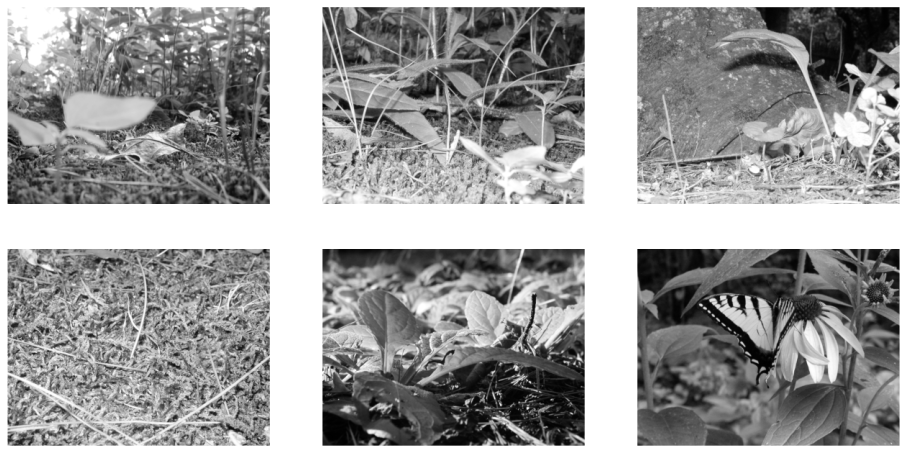
\includegraphics{/Users/bblais/Documents/Git/Amblyopia-Simulation/Manuscript/resources/fig-orig.svg}
\caption{Original natural images.}\label{fig:orig}
}
\end{figure}

\begin{figure}
\hypertarget{fig:logdog}{%
\centering
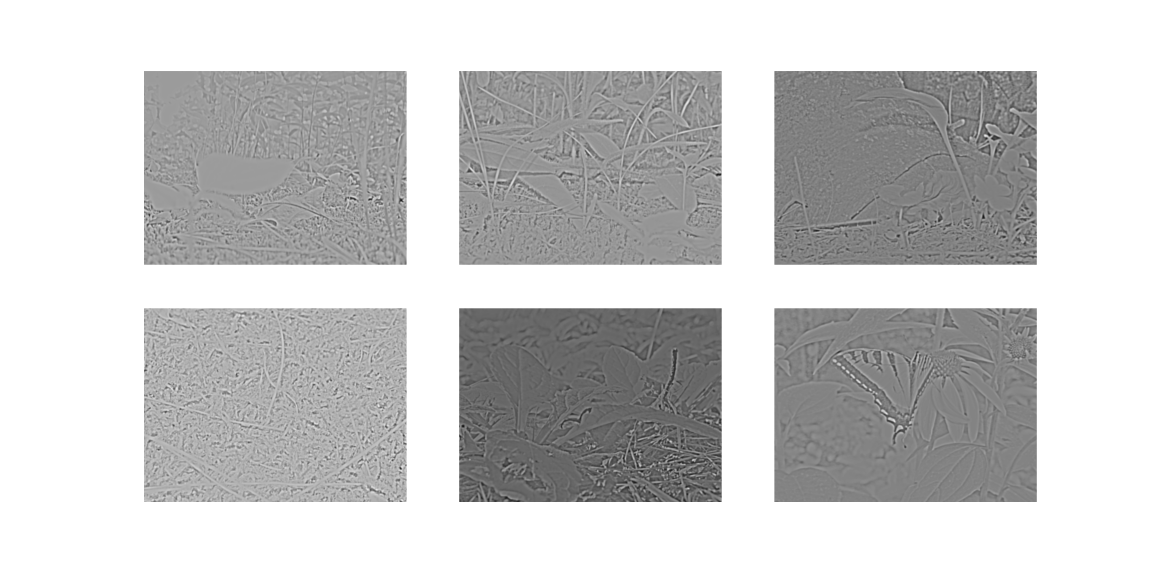
\includegraphics{/Users/bblais/Documents/Git/Amblyopia-Simulation/Manuscript/resources/fig-logdog.svg}
\caption{A Small Subset of the Natural Images filtered with a base-2 Log
function and a difference of Gaussians (DOG)}\label{fig:logdog}
}
\end{figure}

\hypertarget{two-eye-architecture}{%
\subsection{Two-eye architecture}\label{two-eye-architecture}}

Shown in Figure \ref{fig:arch} is the visual field, approximated here as
a two-dimensional projection, to left and right retinal cells. These
left and right retinal cells project to the left and right LGN cells,
respectively, and finally to a single cortical cell. The LGN is assumed
to be a simple relay, and does not modify the incoming retinal activity.
It is important to understand that the model we are pursuing here is a
\emph{single cortical cell} which receives input from both eyes. We will
encounter some limitations to this model which may necessitate exploring
multi-neuron systems.

In the model, normal development is simulated with identical image
patches presented to both eyes combined with small independent noise in
each eye. The random noise is generated from a zero-mean normal
distribution of a particular variance, representing the natural
variation in responses of LGN neurons. Practically, the independent
random noise added to each of the two-eye channels avoids the artificial
situation of having mathematically identical inputs in the channels. The
development of the deficit and the subsequent treatment protocols are
modeled with added preprocessing to these image patches, described later
in \ref{models-of-development-of-amblyopia} and
\ref{models-of-treatments-for-amblyopia}.

For all of the simulations we use a 19x19 receptive field, which is a
compromise between speed of simulation and the limits of spatial
discretization. We perform at least 20 independent simulations for each
condition to address variation in the results.

\begin{figure}
\hypertarget{fig:arch}{%
\centering
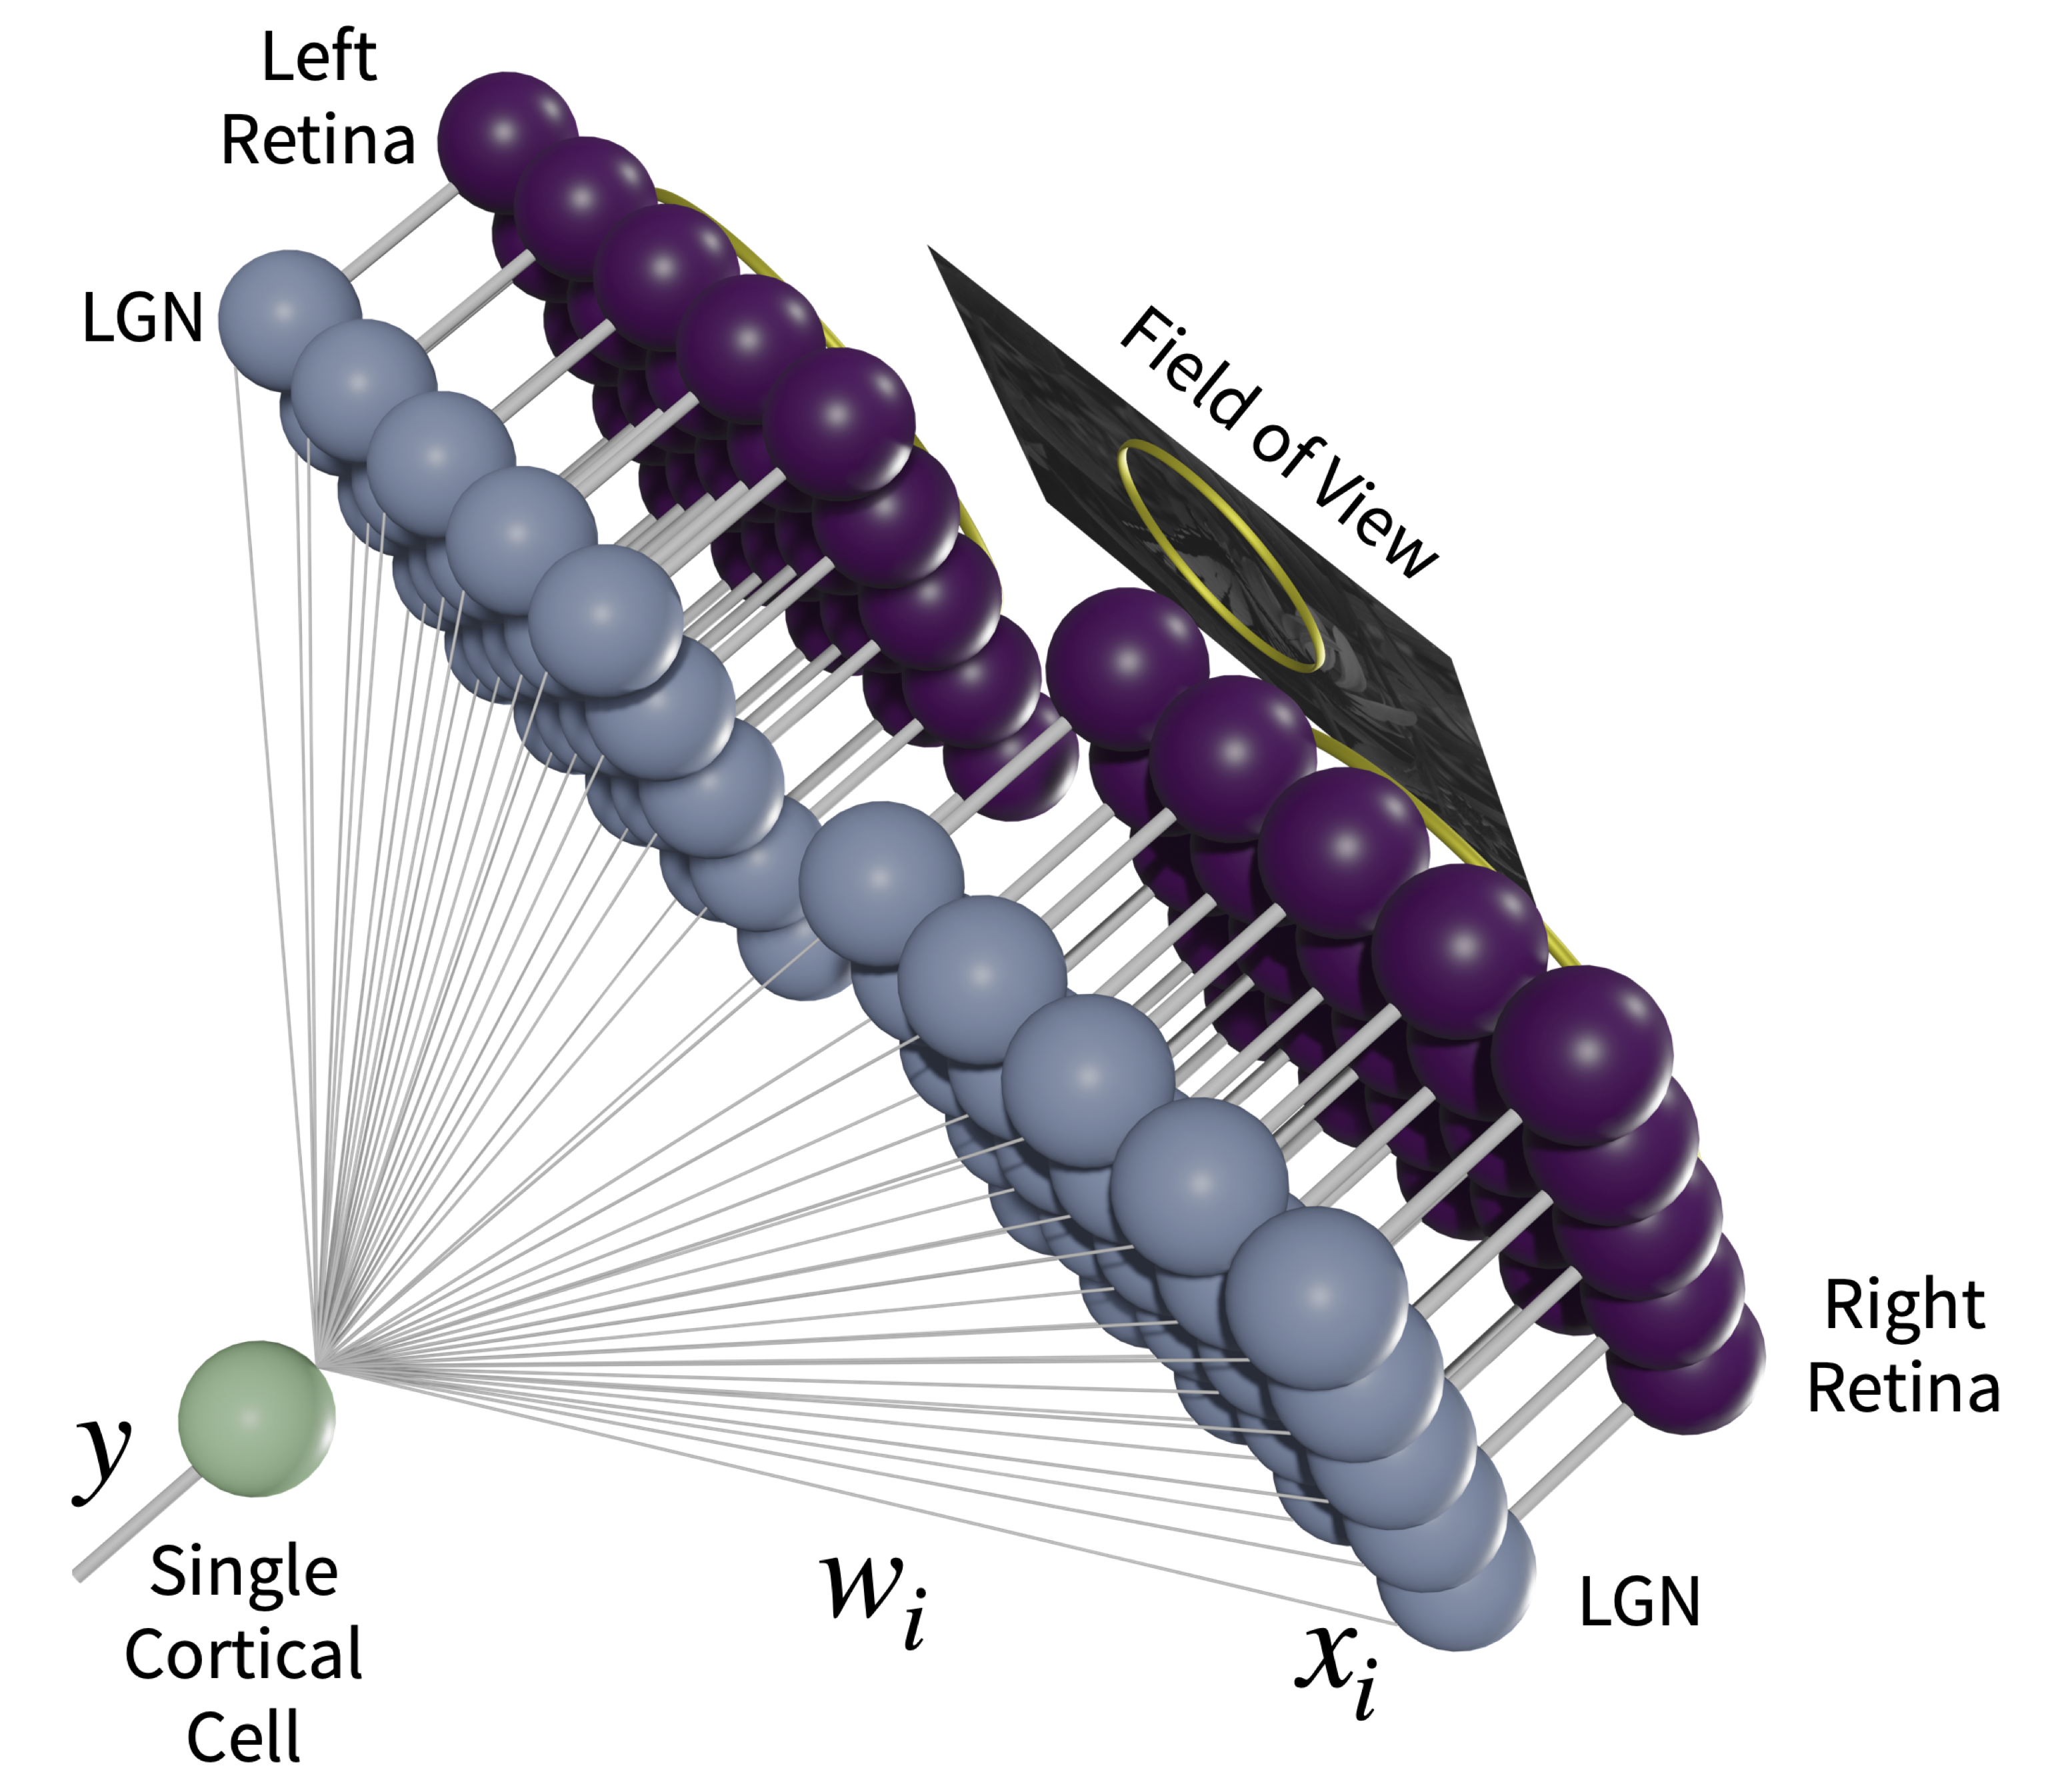
\includegraphics{/Users/bblais/Documents/Git/Amblyopia-Simulation/Manuscript/resources/arch.png}
\caption{Two-eye architecture.}\label{fig:arch}
}
\end{figure}

\begin{figure}
\hypertarget{fig:normal-inputs}{%
\centering
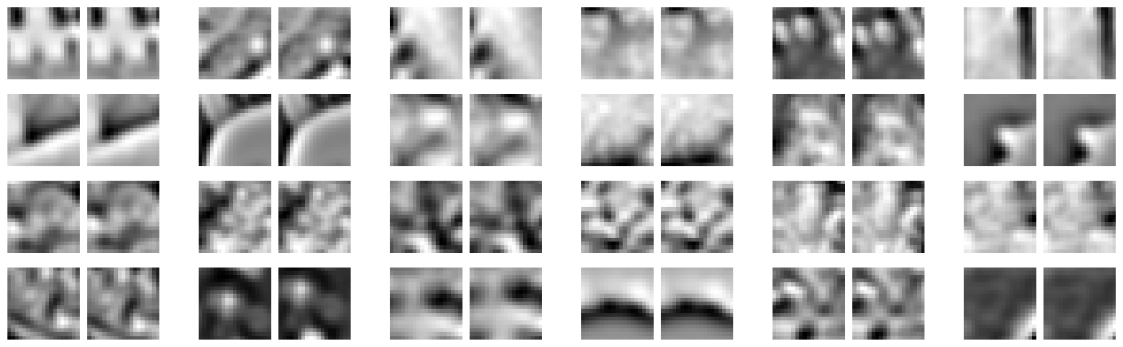
\includegraphics{/Users/bblais/Documents/Git/Amblyopia-Simulation/Manuscript/resources/fig-normal_patches.svg}
\caption{A sample of 24 input patches from a normal visual environment.
The left- and right-eye inputs are shown in
pairs.}\label{fig:normal-inputs}
}
\end{figure}

\hypertarget{synaptic-modification-the-bcm-learning-rule}{%
\subsection{Synaptic Modification: The BCM Learning
Rule}\label{synaptic-modification-the-bcm-learning-rule}}

We use a single neuron and the parabolic form of the BCM(Bienenstock et
al., 1982; Brian S. Blais et al., 2008) learning rule for all of the
simulations, where the synaptic modification depends on the postsynaptic
activity, \(y\), in the following way for a single neuron

\[
y=\sigma\left(\sum_i x_i w_i \right)
\] \[
\frac{dw_i}{dt} = \eta y(y-\theta_M) x_i
\] \[
\frac{d\theta_M}{dt} = (y^2-\theta_M)/\tau
\]

where is \(x_i\) is the \(i\)th presynaptic input, \(w_i\) is the
\(i\)th synaptic weight, and \(y\) is the postsynaptic output activity.
The constant, \(\eta\), refers to the learning rate and the constant,
\(\tau\), is what we call the memory-constant and is related to the
speed of the sliding threshold. The transfer function,
\(\sigma(\cdot)\), places minimum and maximum responses given a set of
inputs and weights.

\begin{figure}
\hypertarget{fig:bcm-phi}{%
\centering
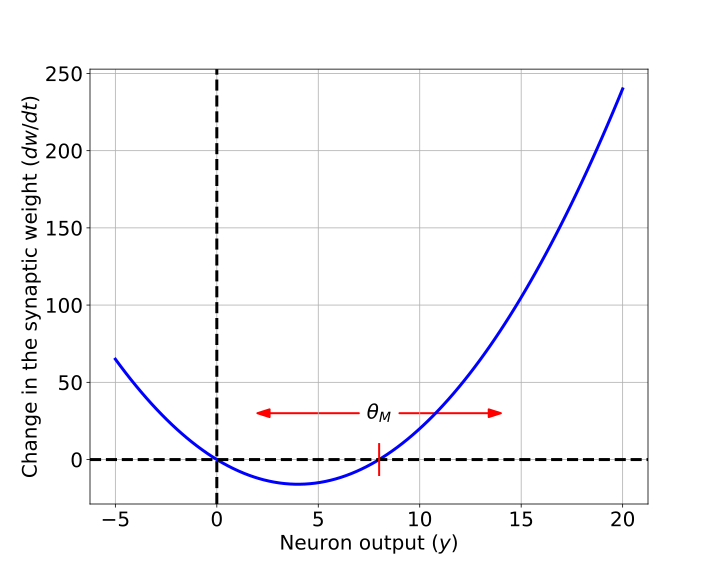
\includegraphics{/Users/bblais/Documents/Git/Amblyopia-Simulation/Manuscript/resources/fig-bcm-phi.svg}
\caption{The BCM synaptic modification function. Units are
arbitrary.}\label{fig:bcm-phi}
}
\end{figure}

The results are extremely robust to values of \(\eta\) and \(\tau\) ,
which are generally chosen for practical, rather than theoretical,
considerations. Each of these constants is related to the time-step for
the simulations, but given the phenomenological nature of the BCM theory
it is beyond the scope of this paper to make detailed comparisons
between simulation time and real-time. Further, the fact that \(\tau\)
can be changed within a factor of 100 with no noticeable effect, the
experiments presented here cannot be used address the time-scales of the
molecular mechanisms underlying synaptic modification. Whenever we refer
to real-time units for a simulation, we approximate a single simulation
iteration as 1 iteration = 0.2 seconds(Brian S. Blais, 1998).

In the BCM learning rule, weights decrease if \(y\) is less than the
modification threshold,\(\theta_M\) , and increase if \(y\) is greater
than the modification threshold. To stabilize learning, the modification
threshold ``slides'' as a super-linear function of the output. The
output, \(y\) , is related to the product of the inputs and the weights
via a sigmoidal function, \(\sigma(\cdot)\), which places constraints on
the values of the output, keeping it in the range -1 and 50. The
interpretation of negative values is consistent with previous work(B. S.
Blais et al., 1998), where the activity values are measured relative to
spontaneous activity. Thus, negative values are interpreted as activity
below spontaneous. We continue this usage, in order to more easily
compare with previous simulations. The role of the spontaneous level for
the simulations in the natural image environment is discussed
elsewhere(B. S. Blais et al., 1998).

\hypertarget{simulation}{%
\subsection{Simulation}\label{simulation}}

The synaptic weights, and the modification threshold, are set to small
random initial values at the beginning of a simulation. At each
iteration, an input patch is generated as described above depending on
the procedure being simulated and then presented to the neuron. After
each input patch is presented, the weights are modified using the output
of the neuron, the input values and the current value of the
modification threshold. In an input environment composed of patches
taken from natural images, with equal patches presented to the left- and
right-eyes as shown in Figure \ref{fig:normal-inputs}, this process
orientation selective and fully binocular cells(B. S. Blais et al.,
1998). We then present test stimulus made from sine-gratings with 24
orientations, 20 spatial frequencies, and optimized over phase. Applying
any of the blur filters to the sine gratings does not quantitatively
change the result.

\begin{figure}
\hypertarget{fig:rf-theta-tuning-curve}{%
\centering
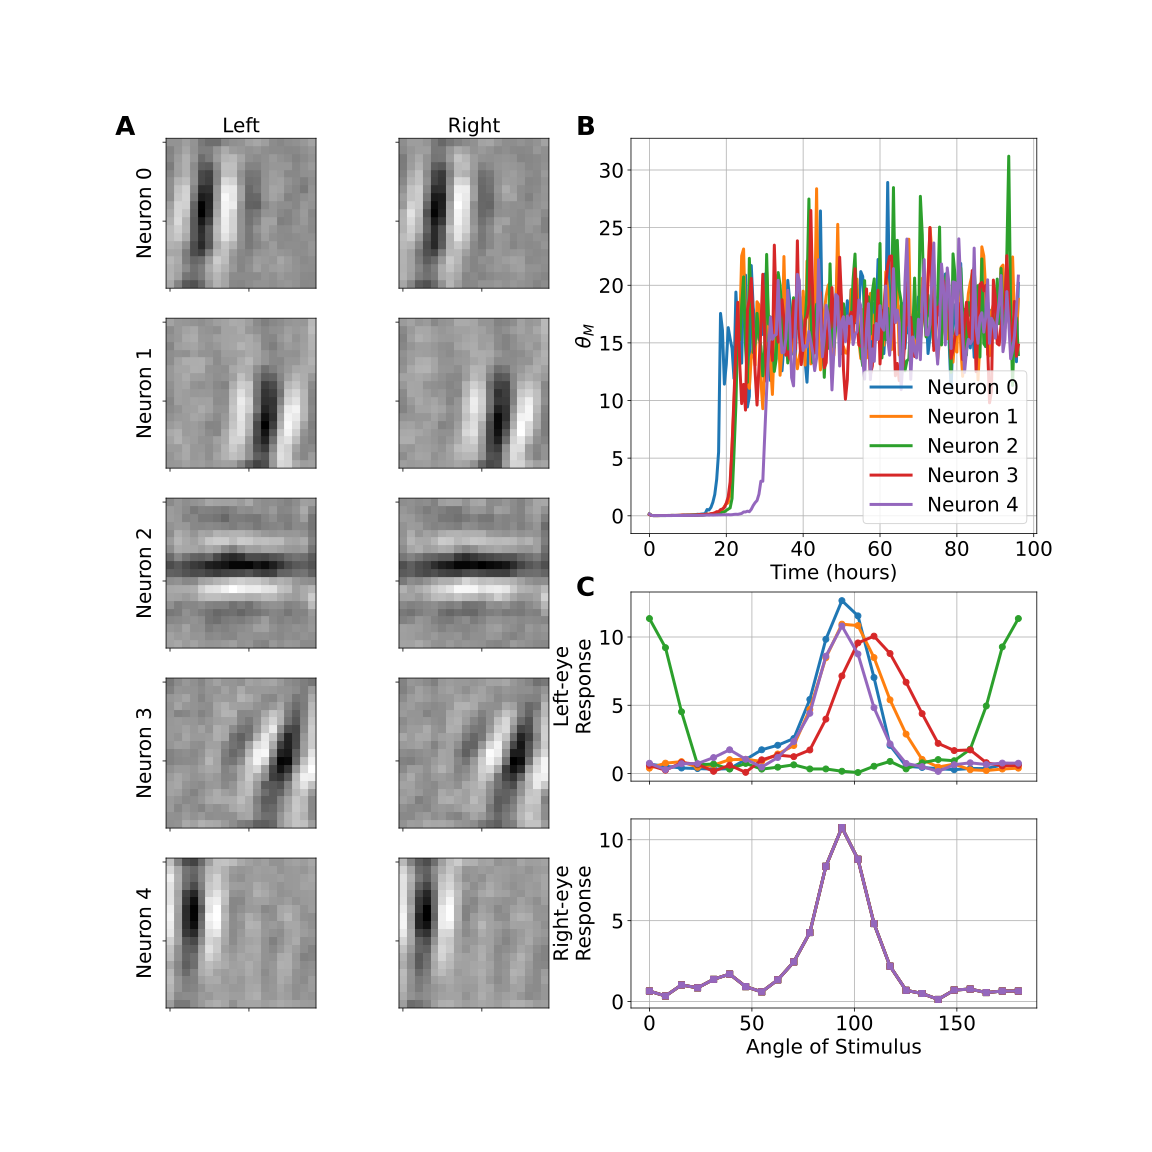
\includegraphics{/Users/bblais/Documents/Git/Amblyopia-Simulation/Manuscript/resources/fig-rf-theta-tuning-curve.svg}
\caption{(A) Synaptic weights where black denotes weak weights and white
denotes strone weights. A clear preference for oriented stimuli can be
seen. (B) BCM modification threshold over time. The value converges to
nearly the same level for all neurons. (C) Responses to Oriented Stimuli
after training. Each neuron develops orientation selectivity to a range
of optimum angles.}\label{fig:rf-theta-tuning-curve}
}
\end{figure}

\hypertarget{models-of-development-of-amblyopia}{%
\subsection{Models of Development of
Amblyopia}\label{models-of-development-of-amblyopia}}

Amblyopia is a reduction of the best-corrected visual acuity (BCVA) with
an otherwise normal eye and has many causes(Wallace et al., 2018). Two
of the most common forms of amblyopia are strabismic and anisometropic
amblyiopia. Strabismic amblyopia occurs when the inputs from each eye do
not converge and the fixating eye becomes dominant over a non-fixating
eye. Refractive amblyopia occurs with untreated unilateral refractive
errors, one kind being anisometropic amblyopia where unequal refractive
power in each eye leads the retinal image from the amblyopic eye to be
blurred relative to the fellow eye. Both of these processes lead to
synaptic plasticity adjustments and interocular competition, enhancing
the initial deficit.

In this work we use a model of the amblyopic deficit caused by two
mechanisms. The first is a blurring of the amblyopic eye inputs,
representing refractive amblyopia. The second is eye-jitter,
representing one source of strabismic amblyopia. We can explore these
mechanisms independently and in conjunction to see how they respond
differentially to the various treatments.

\hypertarget{refractive-amblyopia}{%
\subsubsection{Refractive amblyopia}\label{refractive-amblyopia}}

The amblyopic eye is presented with image patches that have been
\emph{blurred} with a normalized Gaussian filter applied to the images
with a specified width. The larger the width the blurrier the resulting
filtered image. Some examples are shown in Figure
\ref{fig:blurred-inputs}

\begin{figure}
\hypertarget{fig:blurred-inputs}{%
\centering
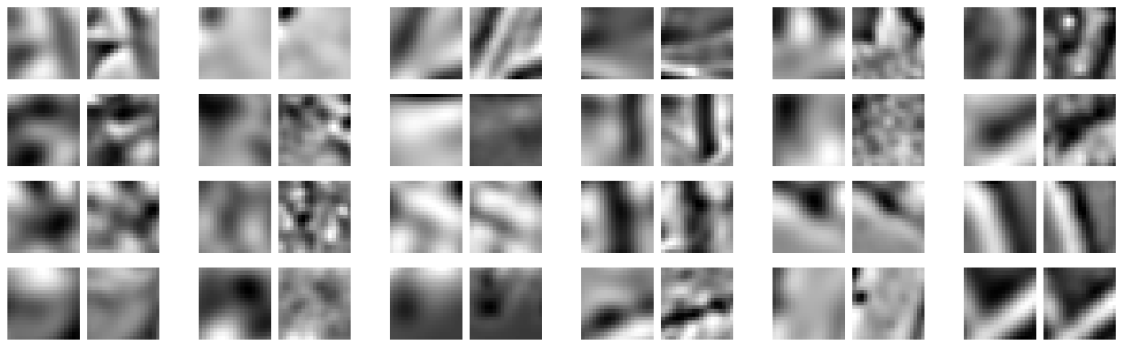
\includegraphics{/Users/bblais/Documents/Git/Amblyopia-Simulation/Manuscript/resources/fig-blurred-inputs.svg}
\caption{A sample of 24 input patches from a refractive amblyopic
environment. The amblyopic (blurred) input is the square on the
left-hand side of each pair.}\label{fig:blurred-inputs}
}
\end{figure}

\hypertarget{strabismic-amblyopia}{%
\subsubsection{Strabismic amblyopia}\label{strabismic-amblyopia}}

Strabismic inputs are modeled by changing the center of the left- and
right-input patches in a systematic way, with a set mean offset and a
standard deviation per input patch generated. In this way we can model
completely overlapping (i.e.~normal) inputs, completely non-overlapping
(i.e.~extreme strabismus), and any amount of overlap in between. Some
examples are shown in Figure \ref{fig:jitter-inputs} with the offset
locations shown in Figure \ref{fig:jitter-input-locations}.

\begin{figure}
\hypertarget{fig:jitter-inputs}{%
\centering
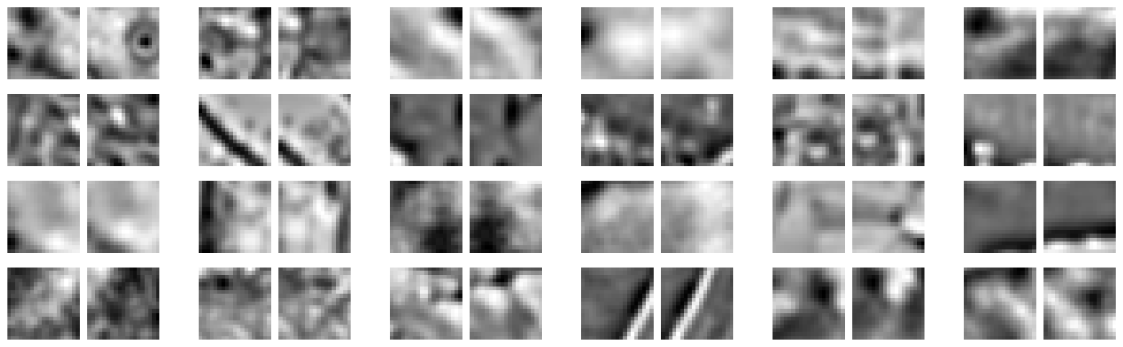
\includegraphics{/Users/bblais/Documents/Git/Amblyopia-Simulation/Manuscript/resources/fig-jitter-inputs.svg}
\caption{A sample of 24 input patches from a strabismic visual
environment achieved through random jitter of the amblyopic (left)
eye.}\label{fig:jitter-inputs}
}
\end{figure}

\begin{figure}
\hypertarget{fig:jitter-input-locations}{%
\centering
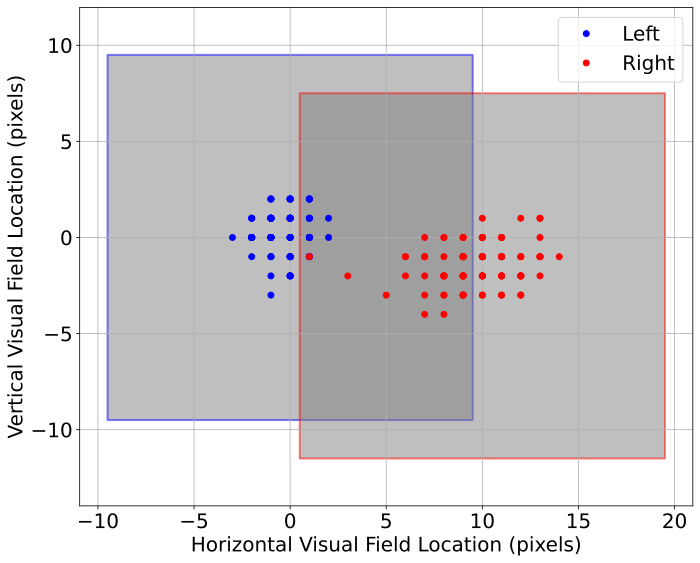
\includegraphics{/Users/bblais/Documents/Git/Amblyopia-Simulation/Manuscript/resources/fig-jitter-locations.svg}
\caption{Locations of the center of the left- and right-field of view
receptive fields, jittered randomly with set mean and standard
deviation. The average receptive fields are shown as gray
squares.}\label{fig:jitter-input-locations}
}
\end{figure}

\hypertarget{models-of-treatments-for-amblyopia}{%
\subsection{Models of Treatments for
Amblyopia}\label{models-of-treatments-for-amblyopia}}

To model the fix to the refractive imbalance we follow the deficit
simulation with an input environment that is rebalanced, both eyes
receiving nearly identical input patches (\ref{fig:normal-inputs}). This
process is a model of the application of refractive correction. Although
both eyes receive nearly identical input patches, we add independent
Gaussian noise to each input channel to represent the natural variation
in the activity in each eye. In addition, in those cases where use
employ strabismic amblyopia, the inter-eye jitter is not corrected with
the refractive correction.

\hypertarget{patch-treatment}{%
\subsubsection{Patch treatment}\label{patch-treatment}}

The typical patch treatment is done by depriving the strong-eye of input
with an eye-patch. In the model this is equivalent to presenting the
strong-eye with random noise instead of the natural image input.
Competition between the left- and right-channels drives the recovery,
and is produced from the difference between \emph{structured} input into
the weak-eye and the \emph{unstructured} (i.e.~noise) input into the
strong eye. It is not driven by a reduction in input activity.
\ref{fig:patch-inputs} shows sample simulation input patterns from the
patched eye. Compare this to \ref{fig:normal-inputs} to see that the
simulated patch has far less structure than the normal inputs.

\begin{figure}
\hypertarget{fig:patch-inputs}{%
\centering
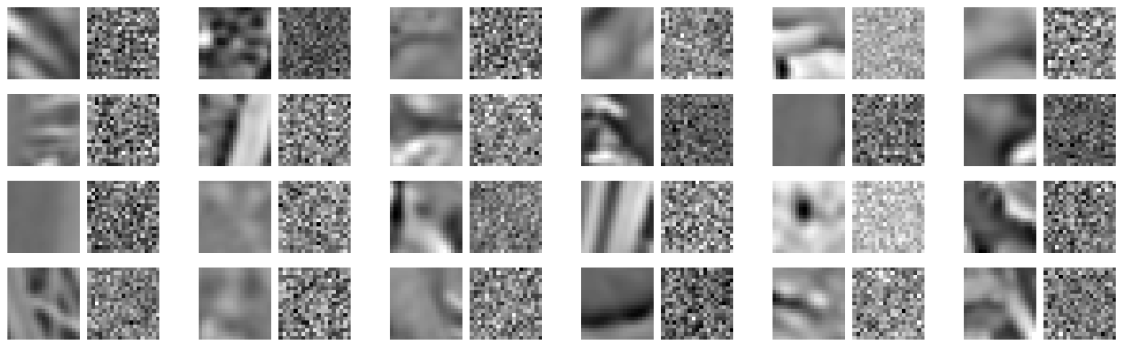
\includegraphics{/Users/bblais/Documents/Git/Amblyopia-Simulation/Manuscript/resources/fig-patch-inputs.svg}
\caption{A sample of 24 input patches from a patched visual
environment.}\label{fig:patch-inputs}
}
\end{figure}

\hypertarget{contrast-modification}{%
\subsubsection{Contrast modification}\label{contrast-modification}}

A binocular approach to treatment can be produced with contrast
reduction of the non-deprived channel relative to the deprived channel.
Experimentally this can be accomplished with VR headsets(Xiao et al.,
2020). In the model we implement this by down-scaling the normal,
unblurred channel with a simple scalar multiplier applied to each pixel.
The contrast difference sets up competition between the two channels
with the advantage given to the weak-eye channel.

\begin{figure}
\hypertarget{fig:contrast-modified-inputs}{%
\centering
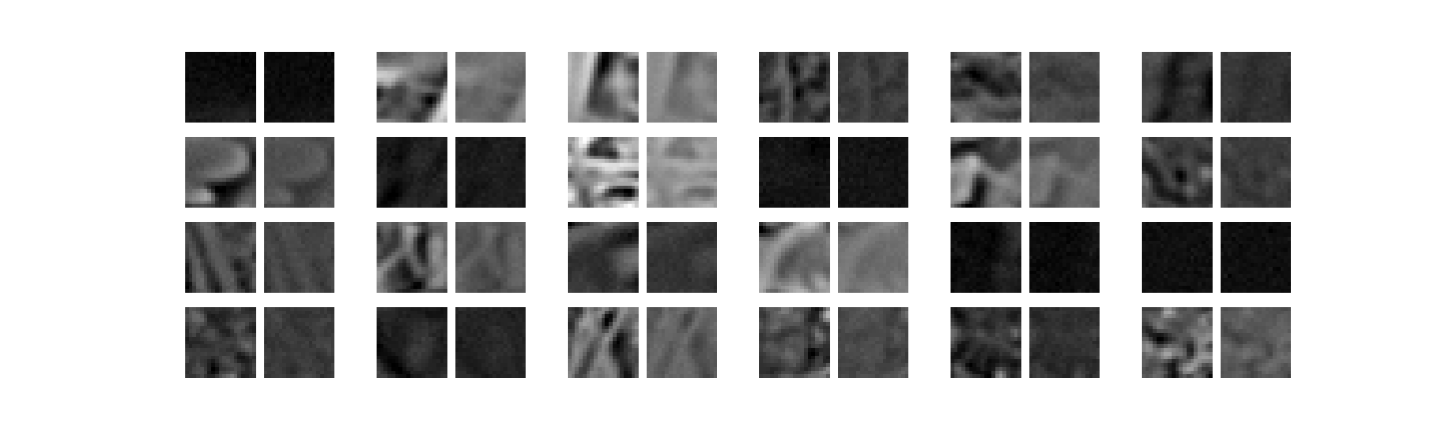
\includegraphics{/Users/bblais/Documents/Git/Amblyopia-Simulation/Manuscript/resources/fig-contrast-modified-inputs.svg}
\caption{A sample of 24 input patches from a normal visual environment
with the right-channel down-scaled relative to the
left.}\label{fig:contrast-modified-inputs}
}
\end{figure}

\hypertarget{dichoptic-masks}{%
\subsubsection{Dichoptic Masks}\label{dichoptic-masks}}

On top of the contrast modification, we can include the application of
the dichoptic mask. In this method, each eye receives a version of the
input images filtered through independent masks in each channel,
resulting in a mostly-independent pattern in each channel. It has been
observed that contrast modification combined with dichoptic masks can be
an effective treatment for amblyopia(Li et al., 2015; Xiao et al.,
2022). The motivation behind the application of the mask filter is that
the neural system must use both channels to reconstruct the full image
and thus may lead to enhanced recovery.

The dichoptic masks are constructed with the following procedure. A
blank image (i.e.~all zeros) is made to which is added 15 randomly sized
circles with values equal to 1 (Figure \ref{fig:dichopic_blob} A). These
images are then smoothed with a Gaussian filter of a given width, \(f\)
(Figure \ref{fig:dichopic_blob} B). This width is a parameter we can
vary to change the overlap between the left- and right-eye images. A
high value of \(f\) compared with the size of the receptive field,
e.g.~\(f=90\), yields a high overlap between the patterns in the weak-
and strong-eye inputs (Figure \ref{fig:dichopic_filter_size}). Likewise,
a small value of \(f\), e.g.~\(f=10\), the eye inputs are nearly
independent -- the patterned activity falling mostly on one of the eyes
and not much to both. Finally, the smoothed images are scaled to have
values from a minimum of 0 to a maximum of 1. This image-mask we will
call \(A\), and is the left-eye mask whereas the right-eye mask, \(F\),
is the inverse of the left-eye mask, \(F\equiv 1-A\). The mask is
applied to an image by multiplying the left- and right-eye images by the
left- and right-eye masks, respectively, resulting in a pair of images
which have no overlap at the peaks of each mask, and nearly equal
overlap in the areas of the images where the masks are near 0.5 (Figure
\ref{fig:dichopic_filter_image}).

\begin{figure}
\hypertarget{fig:dichopic_blob}{%
\centering
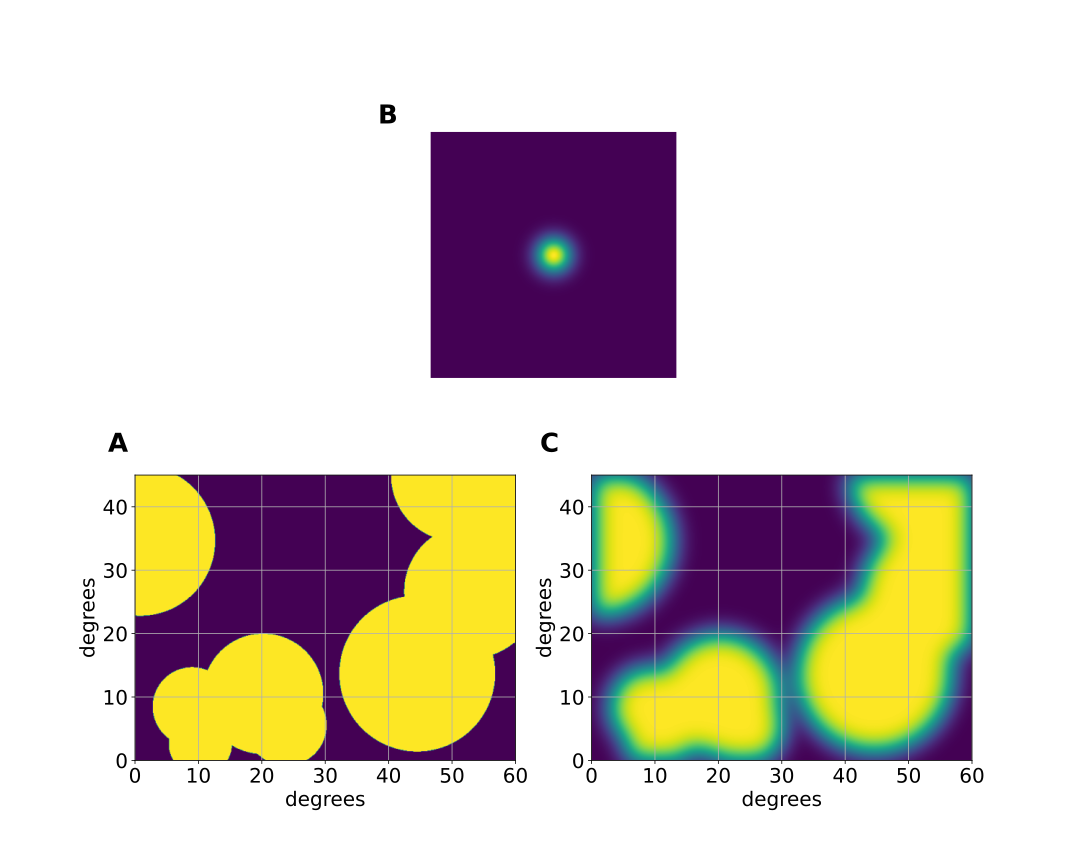
\includegraphics{/Users/bblais/Documents/Git/Amblyopia-Simulation/Manuscript/resources/blob_convolution_example_fsig_20.svg}
\caption{The dichoptic masks are produced by taking random circular
blobs (A), convolving them a Gaussian filter of a specified size (B),
resulting in the circular blobs blending into the background smoothly at
the edges on the scale of the filter (C)}\label{fig:dichopic_blob}
}
\end{figure}

\begin{figure}
\hypertarget{fig:dichopic_filter_size}{%
\centering
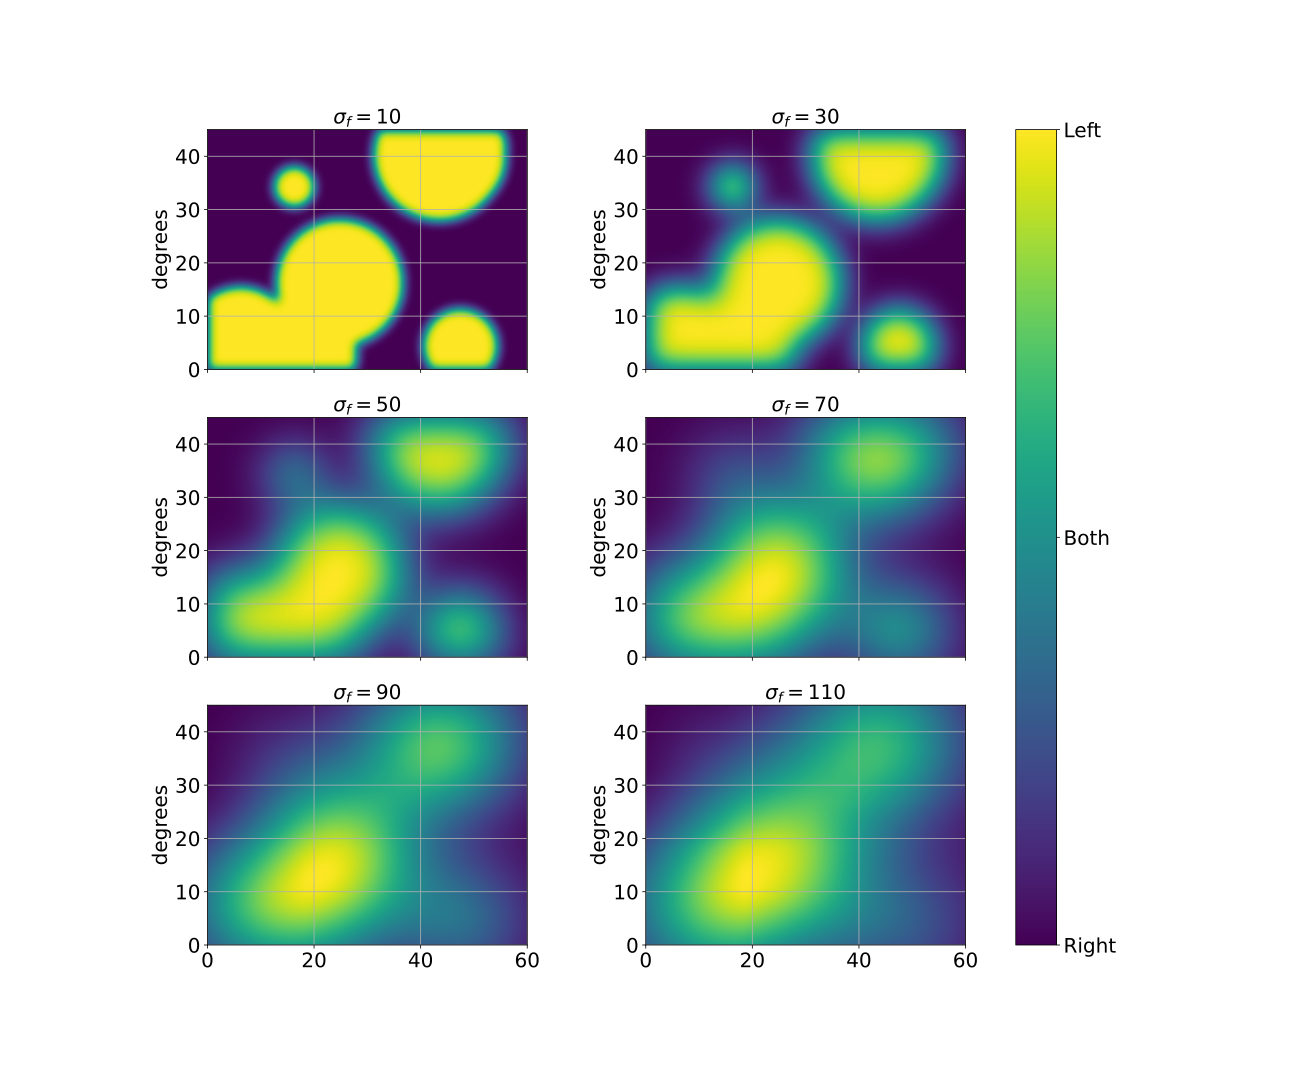
\includegraphics{/Users/bblais/Documents/Git/Amblyopia-Simulation/Manuscript/resources/mask_filter_examples_fsigs.svg}
\caption{The dichoptic masks for several different filter sizes. The
larger the filter, the larger the overlap in the patterns presented to
the two eyes. For a very sharp mask (upper left) patterns are nearly all
to either the left or the right eye. For a wide mask (lower right) most
patterns are presented to both eyes.}\label{fig:dichopic_filter_size}
}
\end{figure}

\begin{figure}
\hypertarget{fig:dichopic_filter_image}{%
\centering
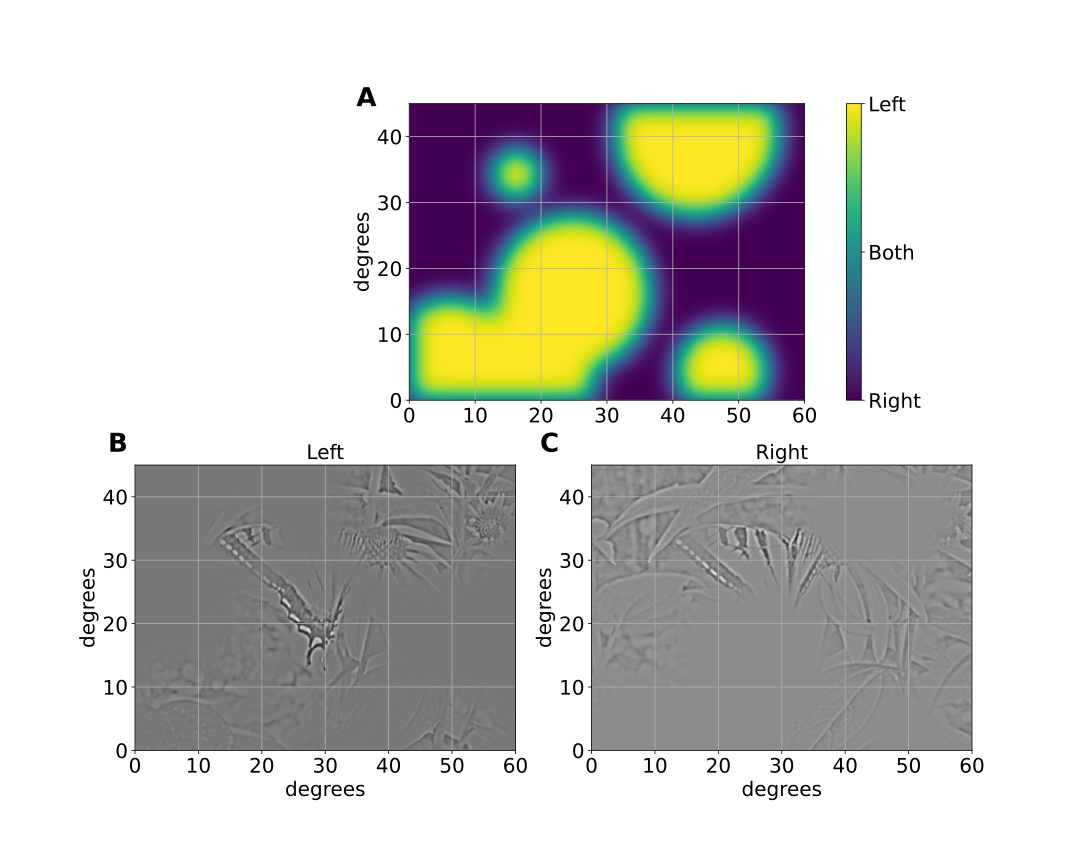
\includegraphics{/Users/bblais/Documents/Git/Amblyopia-Simulation/Manuscript/resources/mask_filter_example_fsig_20.svg}
\caption{An example of a dichoptic mask, \(\sigma = 20\), applied to one
of the images. The mask (A) shows how much of the input goes to each of
the left and right channels. The resulting left- and right-images (B and
C, respectively) show the results of the partial independence of the two
channels. One can see areas where there is some overlap as well as areas
where the pattern is only present in one of the eyes due to the
application of the mask.}\label{fig:dichopic_filter_image}
}
\end{figure}

\hypertarget{atropine-treatment}{%
\subsubsection{Atropine treatment}\label{atropine-treatment}}

In the atropine treatment for amblyopia(Glaser et al., 2002), eye-drops
of atropine are applied to the strong-eye resulting in blurred vision in
that eye. Here we use the same blurred filter used to obtain the deficit
(possibly with a different width) applied to the strong eye (Figure
\ref{fig:atropine-inputs}). The difference in sharpness between the
strong-eye inputs and the weak-eye inputs sets up competition between
the two channels with the advantage given to the weak-eye.

\begin{figure}
\hypertarget{fig:atropine-inputs}{%
\centering
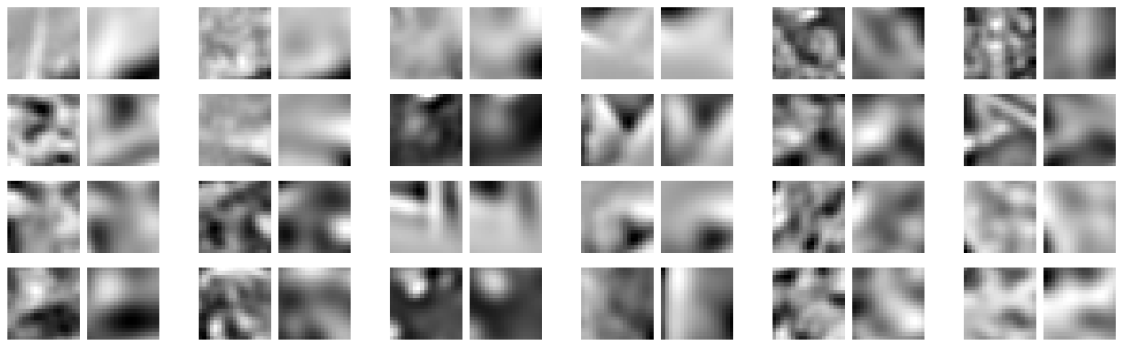
\includegraphics{/Users/bblais/Documents/Git/Amblyopia-Simulation/Manuscript/resources/fig-atropine-inputs.svg}
\caption{A sample of 24 input patches from an environment with atropine
applied to the right eye.}\label{fig:atropine-inputs}
}
\end{figure}

\hypertarget{quantifying-responses}{%
\subsection{Quantifying responses}\label{quantifying-responses}}

\hypertarget{ocular-dominance-index}{%
\subsubsection{Ocular Dominance Index}\label{ocular-dominance-index}}

Simulations are ended when selectivity has been achieved and the
responses are stable. From the maximal responses of each eye,
\(R_{\text{left}}\) and \(R_{\text{right}}\), individually, we can
calculate the ocular dominance index as \[
\text{ODI} \equiv \frac{R_{\text{right}}-R_{\text{left}}}{R_{\text{right}}+R_{\text{left}}}
\] The ocular dominance index (ODI) has a value of
\(\text{ODI} \approx 1\) when stimulus to the right-eye (typically the
strong eye in the simulations, by convention) yields a maximum neuronal
response with little or no contribution from the left-eye. Likewise, an
ocular dominance index (ODI) has a value of \(\text{ODI} \approx -1\)
when stimulus to the left-eye (typically the weak eye, by convention)
yields a maximum neuronal response with little or no contribution from
the right-eye. A value of \(\text{ODI} \approx 0\) represents a purely
binocular cell, responding equally to stimulus in either eye.

\hypertarget{results}{%
\section{Results}\label{results}}

\hypertarget{refractory-and-strabismic-amblyopia}{%
\subsection{Refractory and Strabismic
Amblyopia}\label{refractory-and-strabismic-amblyopia}}

Figure \ref{fig:deficit-mu_c-blur} shows the production of a deficit
effect using both refractory blurring and inter-eye jitter.
Interestingly the larger jitter offset, for small amounts of blur,
reduces both the deficit. While both variables increase the ODI shift to
the stronger eye, the jitter has a more modest effect (Figure
\ref{fig:deficit-ODI-mu_c-blur}).

\begin{figure}
\hypertarget{fig:deficit-mu_c-blur}{%
\centering
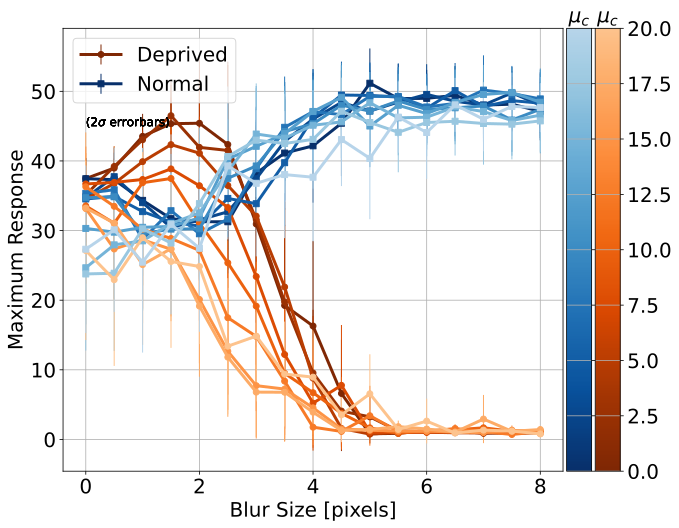
\includegraphics{/Users/bblais/Documents/Git/Amblyopia-Simulation/Manuscript/resources/fig-deficit-mu_c-blur.svg}
\caption{Maximum response for the deprived- and normal-input channels as
function of the deficit blur size (in pixels) and the mean jitter offset
(\(\mu_c\)). Interestingly the larger jitter offset, for small amounts
of blur, reduces both the deficit.}\label{fig:deficit-mu_c-blur}
}
\end{figure}

\begin{figure}
\hypertarget{fig:deficit-ODI-mu_c-blur}{%
\centering
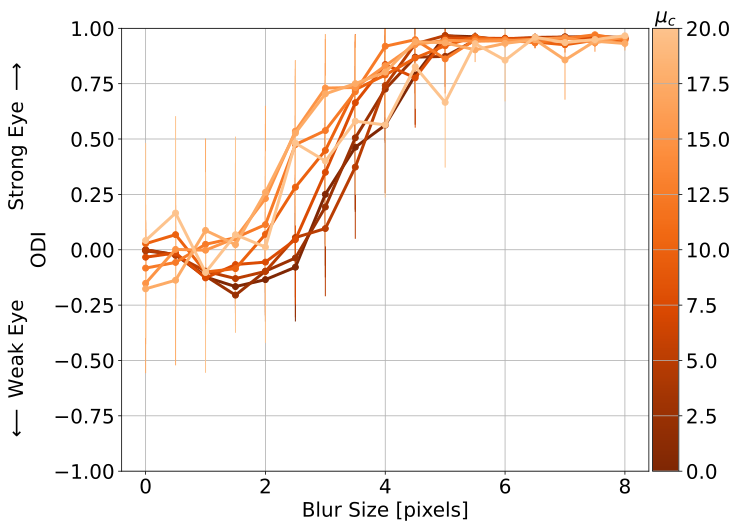
\includegraphics{/Users/bblais/Documents/Git/Amblyopia-Simulation/Manuscript/resources/fig-deficit-ODI-mu_c-blur.svg}
\caption{Ocular dominance index (ODI) as function of the deficit blur
size (in pixels) and the mean jitter offset (\(\mu_c\)). Both variables
increase the ODI shift to the stronger eye, but the jitter has a more
modest effect.}\label{fig:deficit-ODI-mu_c-blur}
}
\end{figure}

\hypertarget{conclusions-and-discussion}{%
\subsection{Conclusions and
Discussion}\label{conclusions-and-discussion}}

\hypertarget{references}{%
\section*{References}\label{references}}
\addcontentsline{toc}{section}{References}

\hypertarget{refs}{}
\begin{CSLReferences}{1}{0}
\leavevmode\vadjust pre{\hypertarget{ref-BCM82}{}}%
Bienenstock, E. L., Cooper, L. N., and Munro, P. W. (1982). Theory for
the development of neuron selectivity: Orientation specificity and
binocular interaction in visual cortex. \emph{Journal of Neuroscience},
\emph{2}, 32--48.

\leavevmode\vadjust pre{\hypertarget{ref-birch2013amblyopia}{}}%
Birch, E. E. (2013). Amblyopia and binocular vision. \emph{Progress in
Retinal and Eye Research}, \emph{33}, 67--84.

\leavevmode\vadjust pre{\hypertarget{ref-phd:Blais98}{}}%
Blais, Brian S. (1998, May). \emph{The role of the environment in
synaptic plasticity:\\
towards an understanding of learning and memory} (PhD thesis). Brown
University, Institute for Brain; Neural Systems; Dr. Leon N Cooper,
Thesis Supervisor.

\leavevmode\vadjust pre{\hypertarget{ref-Blais:2008kx}{}}%
Blais, Brian S., Frenkel, M. Y., Kuindersma, S. R., Muhammad, R.,
Shouval, H. Z., Cooper, L. N., and Bear, M. F. (2008).
\href{https://doi.org/10.1152/jn.90411.2008}{Recovery from monocular
deprivation using binocular deprivation}. \emph{J Neurophysiol},
\emph{100}(4), 2217--24.

\leavevmode\vadjust pre{\hypertarget{ref-BlaisEtAl98}{}}%
Blais, B. S., Intrator, N., Shouval, H., and Cooper, L. N. (1998).
Receptive field formation in natural scene environments: Comparison of
single cell learning rules. \emph{Neural Computation}, \emph{10}(7),
1797--1813.

\leavevmode\vadjust pre{\hypertarget{ref-Gao_2018}{}}%
Gao, T. Y., Guo, C. X., Babu, R. J., Black, J. M., Bobier, W. R.,
Chakraborty, A., \ldots{} al., et. (2018).
\href{https://doi.org/10.1001/jamaophthalmol.2017.6090}{Effectiveness of
a binocular video game vs placebo video game for improving visual
functions in older children, teenagers, and adults with amblyopia}.
\emph{JAMA Ophthalmology}, \emph{136}(2), 172.

\leavevmode\vadjust pre{\hypertarget{ref-glaser2002randomized}{}}%
Glaser, S. R., Matazinski, A. M., Sclar, D. M., Sala, N. A., Vroman, C.
M., Tanner, C. E., et al.others. (2002). A randomized trial of atropine
vs patching for treatment of moderate amblyopia in children.
\emph{Archives of Ophthalmology}, \emph{120}(3), 268--278.

\leavevmode\vadjust pre{\hypertarget{ref-Holmes_2016}{}}%
Holmes, Jonathan M., Manh, V. M., Lazar, E. L., Beck, R. W., Birch, E.
E., Kraker, R. T., \ldots{} al., et. (2016a).
\href{https://doi.org/10.1001/jamaophthalmol.2016.4262}{Effect of a
binocular iPad game vs part-time patching in children aged 5 to 12 years
with amblyopia}. \emph{JAMA Ophthalmology}, \emph{134}(12), 1391.

\leavevmode\vadjust pre{\hypertarget{ref-holmes2016randomized}{}}%
Holmes, Jonathan M., Manh, V. M., Lazar, E. L., Beck, R. W., Birch, E.
E., Kraker, R. T., et al.others. (2016b). A randomized trial of a
binocular iPad game versus part-time patching in children 5 to 12 years
of age with amblyopia. \emph{JAMA Ophthalmology}, \emph{134}(12), 1391.

\leavevmode\vadjust pre{\hypertarget{ref-hubel1995eye}{}}%
Hubel, D. H. (1995). \emph{Eye, brain, and vision.} Scientific American
Library/Scientific American Books.

\leavevmode\vadjust pre{\hypertarget{ref-JeonEtAl1998}{}}%
Jeon, C. J., Strettoi, E., and Masland, R. H. (1998). {The major cell
populations of the mouse retina}. \emph{J Neurosci}, \emph{18}(21),
8936--8946.

\leavevmode\vadjust pre{\hypertarget{ref-Kelly_2016}{}}%
Kelly, K. R., Jost, R. M., Dao, L., Beauchamp, C. L., Leffler, J. N.,
and Birch, E. E. (2016).
\href{https://doi.org/10.1001/jamaophthalmol.2016.4224}{Binocular iPad
game vs patching for treatment of amblyopia in children}. \emph{JAMA
Ophthalmology}, \emph{134}(12), 1402.

\leavevmode\vadjust pre{\hypertarget{ref-Li:2015aa}{}}%
Li, S. L., Reynaud, A., Hess, R. F., Wang, Y.-Z., Jost, R. M., Morale,
S. E., \ldots{} Birch, E. E. (2015).
\href{https://doi.org/10.1016/j.jaapos.2015.08.003}{Dichoptic movie
viewing treats childhood amblyopia}. \emph{J AAPOS}, \emph{19}(5),
401--5.

\leavevmode\vadjust pre{\hypertarget{ref-SterlingEtAl1988}{}}%
Sterling, P., Freed, M. A., and Smith, R. G. (1988). {Architecture of
rod and cone circuits to the on-beta ganglion cell}. \emph{J Neurosci},
\emph{8}(2), 623--642.

\leavevmode\vadjust pre{\hypertarget{ref-wallace2018amblyopia}{}}%
Wallace, D. K., Repka, M. X., Lee, K. A., Melia, M., Christiansen, S.
P., Morse, C. L., and Sprunger, D. T. (2018). Amblyopia preferred
practice pattern{\textregistered}. \emph{Ophthalmology}, \emph{125}(1),
P105--P142.

\leavevmode\vadjust pre{\hypertarget{ref-xiao2022randomized}{}}%
Xiao, S., Angjeli, E., Wu, H. C., Gaier, E. D., Gomez, S., Travers, D.
A., et al.others. (2022). Randomized controlled trial of a dichoptic
digital therapeutic for amblyopia. \emph{Ophthalmology}, \emph{129}(1),
77--85.

\leavevmode\vadjust pre{\hypertarget{ref-xiao2020improved}{}}%
Xiao, S., Gaier, E. D., Mazow, M. L., Stout, A. U., Travers, D. A.,
Angjeli, E., \ldots{} Hunter, D. G. (2020). Improved adherence and
treatment outcomes with an engaging, personalized digital therapeutic in
amblyopia. \emph{Scientific Reports}, \emph{10}(1), 1--8.

\leavevmode\vadjust pre{\hypertarget{ref-de2007current}{}}%
Zárate, B. R. de, and Tejedor, J. (2007). Current concepts in the
management of amblyopia. \emph{Clinical Ophthalmology (Auckland, NZ)},
\emph{1}(4), 403.

\end{CSLReferences}

\end{document}
